\addcontentsline{toc}{section}{Materials and Methods}
\section*{Materials and Methods}

%%%%%%%%%%%%%%%%%%%%%%%%%%%%%%%%%%%%%%%%%%%%%%%%%%%%%%%%%%%%%%%%%%%%%%%
\phantomsection
\addcontentsline{toc}{subsection}{Study Site}
\subsection*{Study Site}

\begin{itemize}
    \item 50-ha long term forest monitoring plot
    \item central Panama
    \item (lat, lon)
    \item moist lowland tropical predominantly evergreen forest, only 10\% of canopy drops leaves during the dry season %\citep{condt_2000} 
    \item mean annual precipitation of $2662 \pm 479$ (SD) mm yr$^{(-1)}$ and a 4-month dry season ($<$ 100 mm per month)  
    \item average annual rainfall of about 2640 mm (Detto et al.,
2018) and a well-marked dry season (total rainfall between late-December and mid-April is about 175 mm on average). 
\end{itemize}
%%%%%%%%%%%%%%%%%%%%%%%%%%%%%%%%%%%%%%%%%%%%%%%%%%%%%%%%%%%%%%%%%%%%%%%
\phantomsection
\addcontentsline{toc}{subsubsection}{Initial Vegetation Conditions}
\subsection*{Initial Conditions}

\paragraph{BCI 2012 survey data}
After establishment in 1981 in 1981, species and dbh of all living trees $<$ 1 cm have been inventoried every 5 years since 1985 \citep{condit_1995}. 

\paragraph{Soil} 
Soil data?

%%%%%%%%%%%%%%%%%%%%%%%%%%%%%%%%%%%%%%%%%%%%%%%%%%%%%%%%%%%%%%%%%%%%%%%
\addcontentsline{toc}{subsubsection}{Atmospheric Conditions}
\subsection*{Atmospheric Conditions}

\paragraph{Choosing Simulation Period}

% \begin{wrapfigure}{!r}{0.45\textwidth}
%     \centering
%     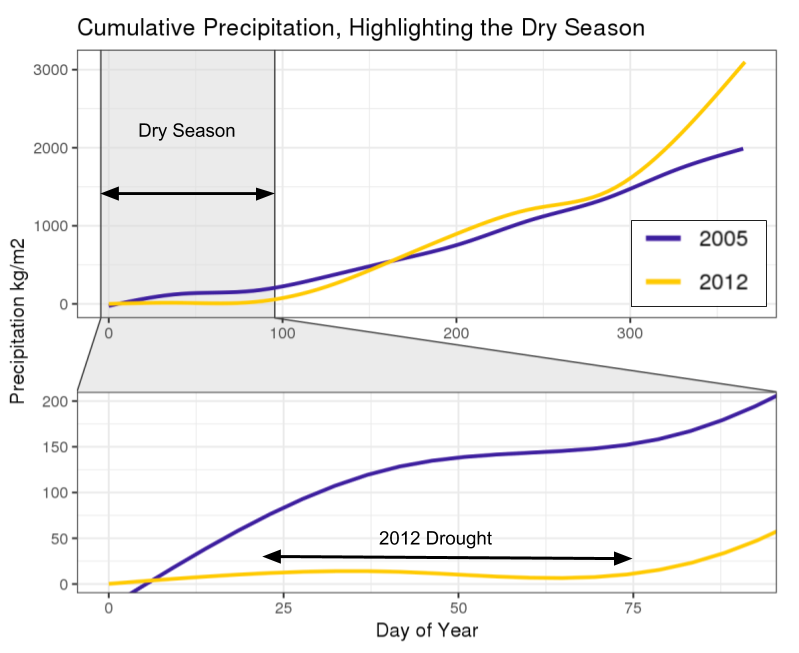
\includegraphics[width=.45\textwidth]{Hydro_Paper_LaTeX/Hydro_Paper_Figures/precip.png}
%     \caption[Precipitation]{Precipitation: To be more informative, this plot should also have the average of all the available years to get a better idea of how "extreme" these two scenarios actually are.}
%     \todoa{caption}
%     \label{fig:precip}
% \end{wrapfigure}

\begin{figure}[!h]
    \centering
    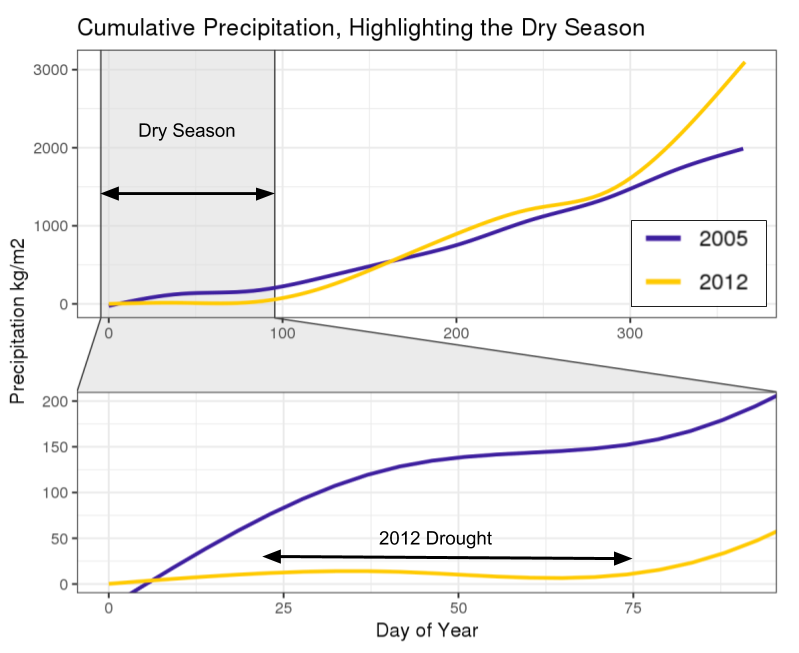
\includegraphics[width=.65\textwidth]{Hydro_Paper_LaTeX/Hydro_Paper_Figures/precip.png}
    \caption[Precipitation]{Cumulative precipitation at Barro Colorado Island, Panama for the years 2012 (yellow) and 2005 (purple). The pictured years have the most divergent climactic conditions over the dry season, with 2012 having an dry and prolonged dry season and 2005 having a short and wet dry season. 
    \todoq{To be more informative, this plot should also have the average of all the available years to get a better idea of how "extreme" these two scenarios actually are.}}
    % \todoa{caption}
    \label{fig:precip}
\end{figure}


For this study we used meteorological seven-year record (2008-2014) of meteorological observations from BCI prepared by \citep{powell_2019}. Data were available at hourly resolution for air temperature, wind speed, specific humidity, precipitation rate, short- and longwave radiation. Because we were focused on processes that took place over a short time scale, we decided to limit runs to one year in length. Two years (\ref{fig:precip}) were chosen to represent climatic extremes in the available data: the shortest and wettest dry season (2005) and the longest and driest dry season (2012). 
 
%%%%%%%%%%%%%%%%%%%%%%%%%%%%%%%%%%%%%%%%%%%%%%%%%%%%%%%%%%%%%%%%%%%%%%%
\addcontentsline{toc}{subsection}{Ecosystem Demography Model Version 2.2}
\subsection*{Ecosystem Demography Model (Version 2.2)}

\begin{figure}[h]
    \centering
    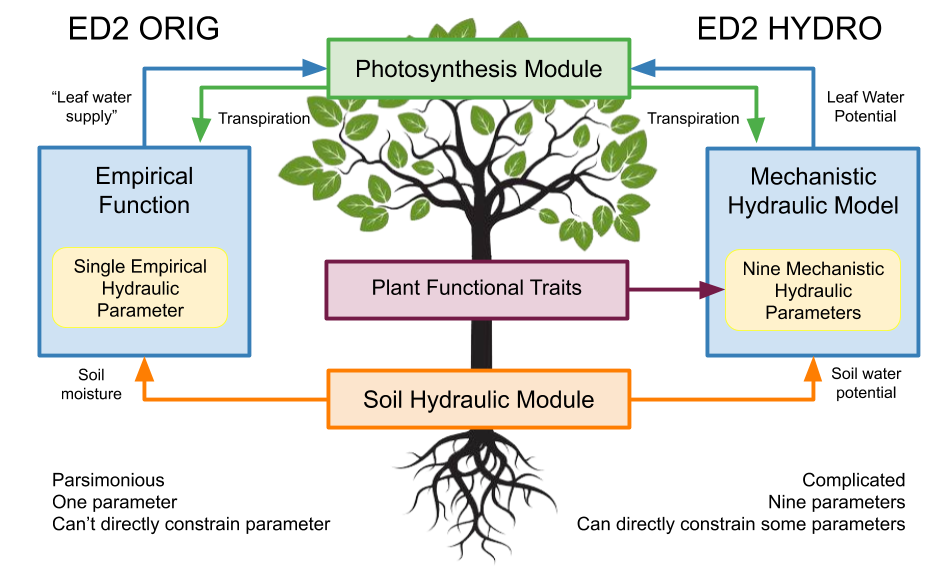
\includegraphics[width=.75\textwidth]{Hydro_Paper_LaTeX/Hydro_Paper_Figures/ED_versions.png}
    \caption[ED2 versions]{ED2 vs ED2-hydro}
    \label{fig:ED_versions}
\end{figure}

ED2 simulates fast time-scale vegetation dynamics using integrated submodels of plant growth and mortality, phenology, disturbance, biodiversity, hydrology, and soil biogeochemistry. In addition, ED2 has been formulated at the scale of individual plants, using a system of size and age structured partial differential equations to dynamically track the behavior of a vertically stratified, spatially distributed ensemble  of individual plants within each climatological grid cell. Because the scope of this study is to focus on the propagation of parameter uncertainly over fast timescale processes, competition between PFTs was not included.



% \begin{itemize}
%     \item 
%     \item ED2-hydro Tropical PFT: http://psql-pecan.bu.edu/bety/pfts/1000000131
%     \item ED2 TropicalPFT: http://psql-pecan.bu.edu/bety/pfts/1000000132
%     \item The PFTs are based on clones of a FATES prior, and then species were added in during the meta-analysis. Should I discuss this process?
% \end{itemize}



%%%%%%%%%%%%%%%%%%%%%%%%%%%%%%%%%%%%%%%%%%%%%%%%%%%%%%%%%%%%%%%%%%%%%%%
%%%%%%%%%%%%%%%%%%%%%%%%%%%%%%%%%%%%%%%%%%%%%%%%%%%%%%%%%%%%%%%%%%%%%%%
\addcontentsline{toc}{subsection}{Attributing Uncertainty to Ecological Processes}
\subsection*{Attributing Uncertainty to Ecological Processes}

\phantomsection
\addcontentsline{toc}{subsubsection}{The Predictive Ecosystem Analyser}
\subsubsection*{PEcAn}

\begin{itemize}
    \item For the purposes of this study, we approach Plant Functional Types (PFTs) by first defining a collection of species. 
    \item These species are cross-listed with a trait database. 
    \item The resulting data can be used to constrain probability distributions that describe our apriori knowledge of the model parameter values for the plant traits in question.
    \item To initialize parameter values for a model run in ED2, a Bayesian meta-analysis is performed in which posterior distributions are calculated for each model parameter  included in the analysis, initial values are randomly selected from the distribution. Note that the out current meta-analyse workflow does not allow for joint distribution sampling. 
    \item One of the benefits of the Bayesian approach to data synthesis is that the posterior distribution can be updated each time new data becomes available. 
    \item This encourages an iterative approach to model-data synthesis in which model uncertainty analysis informs targeted field research which in turn produces data that will be incorporated back in to the Bayesian meta-analysis. \todoc{Davidson 2012? The thesis? This is what Raczka cites when introducing this loop.}
\end{itemize}
 
The Predictive Ecosystem Analyser (PEcAn, \hyperlink{pecanproject.org}{https://pecanproject.github.io/})
is a set of workflows and tools designed to facilitate the full process of interfacing with the Biofuel Ecophysiological Traits and Yield database, or ingesting your own observational data, creating priors, running a Bayesian meta-analysis to produce posterior predictive parameter distributions, sampling from parameter distributions and preparing other model data constraints, running models, processing outputs, validating, benchmarking and running uncertainty analyses. 

\todoq{ \citep{lebauer_2013, raczka_2018, dietze_2017a} all do a very through job of describing how PEcAn calculates parameter uncertainty. It may make sense for me to actually write it down in my own words for the dissertation, but it doesn't really seem necessary for this as a paper.}\todoc{Felicien's paper in review, Dietze 2014}

\paragraph{Meta Analysis}

I started with traits for which I had summary statistics based on expert elicitation (How do I cite that FATES spreadsheet?) Fro each set of data points I found a best fitting distribution from a selection (normal, log normal, Chi Squared, Beta, Poisson, Exponential, Weibull and Uniform,) and entering the priors in to the database.With the priors I constructed using apriori knowledge and I was able to use the process functions from the ED2 hydraulics module to probability density distributions for the remaining hydraulic traits. 


\todoq{
\hyperlink{ED HYDRO DOCUMENTAT}{https://bcow.github.io/ED.Hydro.Documentation}

I have up to date documentation detailing the process of defining the hydraulic trait priors. Not sure how much of this I should include, but it's all there (at least for the hydraulic traits, the rest need to be updated).}

Meta-Analysis Data:
\begin{itemize}
    \item Non-hydraulic trait data: BETYdb \citep{lebauer_2017}
    \item Hydraulic trait data: Verbeek lab paper(s) \todoc{hydraulic meta-analysis which papers?}
    \item Leaf biomass allometry trait data: BAAD database \citep{falster_2015}
    \item Fine root allocation: FRED \citep{iversen_2017}
    \item Root depth allometry \citep{smithmartin_2020}
\end{itemize}

%Please add the following packages if necessary:
%\usepackage{booktabs, multirow} % for borders \& merged ranges
%\usepackage{soul}% for underlines
%\usepackage[table]{xcolor} % for cell colors
%\usepackage{changepage,threeparttable} % for wide tables

%If the table is too wide, replace \begin{table}[!htp]...\end{table} with
%\begin{adjustwidth}{-2.5 cm}{-2.5 cm}\centering\begin{threeparttable}[!htb]...\end{threeparttable}\end{adjustwidth}
\begin{table}[!htp]\centering
\caption{Table of Parameters (Do we want this table to also include distributions?)}\label{tab:params}
\scriptsize
\begin{tabular}{lrrcc|rrrr}\toprule
Trait &Proccess(es) &Units &ED2 &ED2-hydro &Prior distribution &Param a &Param b \\\midrule
Leaf Turgor Loss Point &Hydraulics & &- &+ & & & \\
Leaf Water Cap &Hydraulics & &- &+ & & & \\
Root Beta &Hydraulics & &- &+ & & & \\
Specific Root Area &Hydraulics & &- &+ & & & \\
stoma_psi_c &Hydraulics & &- &+ & & & \\
Kexp &Hydraulics & &- &+ & & & \\
Kmax &Hydraulics & &- &+ & & & \\
Wood Turgor Loss Point &Hydraulics & &- &+ & & & \\
p50 &Hydraulics & &- &+ & & & \\
Wood Water Cap &Hydraulics & &- &+ & & & \\
Water Cond. &Hydraulics & &+ &- & & & \\
Abvgnd \% Struc. Biomass &Allocation \& Allometry & &+ &+ & & & \\
Leaf Biomass Allom. Int. &Allocation \& Allometry & &+ &+ & & & \\
Root Depth Allom. Int. &Allocation \& Allometry & &+ &+ & & & \\
Leaf Biomass Allom. Slope &Allocation \& Allometry & &+ &+ & & & \\
Root Depth Allom. Slope &Allocation \& Allometry & &+ &+ & & & \\
Fine Root Allocation &Allocation \& Allometry & &+ &+ & & & \\
Specific Leaf Area &Allocation \& Allometry & &+ &+ & & & \\
Wood Density &Allocation \& Allometry & &+ &+ & & & \\
Quantum Efficiency &Photosynthesis \& Stomatal Cond. & &+ &+ & & & \\
Stomatal Slope &Photosynthesis \& Stomatal Cond. & &+ &+ & & & \\
Vcmax &Photosynthesis \& Stomatal Cond. & &+ &+ & & & \\
Leaf NIR reflectance &Radiation & &+ &+ & & & \\
Leaf VIS reflectance &Radiation & &+ &+ & & & \\
Leaf NIR transmittance &Radiation & &+ &+ & & & \\
Leaf VIS transmittance &Radiation & &+ &+ & & & \\
Leaf orientation &Radiation & &+ &+ & & & \\
Growth Respiration &Respiration \& Turnover & &+ &+ & & & \\
Leaf Respiration Rate &Respiration \& Turnover & &+ &+ & & & \\
Leaf Turnover Rate &Respiration \& Turnover & &+ &+ & & & \\
Root Turnover Rate &Respiration \& Turnover & &+ &+ & & & \\
Veg. Resp. Q10 &Respiration \& Turnover & &+ &+ & & & \\
\bottomrule
\end{tabular}
\end{table}


\addcontentsline{toc}{subsubsection}{Calculating Parameter Sensitivity and Contribution to Model Uncertainty}
\subsubsection*{Calculating Parameter Sensitivity and Contribution to Model Uncertainty}

\paragraph{Sensitivity Analysis and Variance Decomposition}

\addcontentsline{toc}{subsubsection}{Benchmarking}
\subsubsection*{Benchmarking}

\todoq{
This part of the analysis hasn't really been developed yet. Koven 2020 cites Detto 2018 as having observational eddy-covariance data such as GPP, LH, SH as well as observations of LAI.

Some form of model validation would be important to show that ED2-hydro is in fact making reasonable predictions while simultaneously reducing predictive variability. However, especially given \citep{powell_2018} showing the strength in ED2-hydro's predictive performance at this very site, I don't feel a particular need to spend a lot of time on benchmarking in this paper (also this takes time!). I'd like to hear other opinions on this. }